%package list
\documentclass{article}
\usepackage[top=3cm, bottom=3cm, outer=3cm, inner=3cm]{geometry}
\usepackage{multicol}
\usepackage{graphicx}
\usepackage{url}
%\usepackage{cite}
\usepackage{hyperref}
\usepackage{array}
%\usepackage{multicol}
\newcolumntype{x}[1]{>{\centering\arraybackslash\hspace{0pt}}p{#1}}
\usepackage{natbib}
\usepackage{pdfpages}
\usepackage{multirow}
\usepackage[normalem]{ulem}
\useunder{\uline}{\ul}{}
\usepackage{svg}
\usepackage{xcolor}
\usepackage{listings}
\lstdefinestyle{ascii-tree}{
    literate={├}{|}1 {─}{--}1 {└}{+}1 
  }
\lstset{basicstyle=\ttfamily,
  showstringspaces=false,
  commentstyle=\color{red},
  keywordstyle=\color{blue}
}
%\usepackage{booktabs}
\usepackage{caption}
\usepackage{subcaption}
\usepackage{float}
\usepackage{array}

\newcolumntype{M}[1]{>{\centering\arraybackslash}m{#1}}
\newcolumntype{N}{@{}m{0pt}@{}}


%%%%%%%%%%%%%%%%%%%%%%%%%%%%%%%%%%%%%%%%%%%%%%%%%%%%%%%%%%%%%%%%%%%%%%%%%%%%
%%%%%%%%%%%%%%%%%%%%%%%%%%%%%%%%%%%%%%%%%%%%%%%%%%%%%%%%%%%%%%%%%%%%%%%%%%%%
\newcommand{\itemEmail}{mvelasquea@unsa.edu.pe}
\newcommand{\itemStudent}{Mikhail Gabino Velasque Arcos}
\newcommand{\itemCourse}{Laboratorio FUNDAMENTOS DE LA PROGRAMACION II}
\newcommand{\itemCourseCode}{20214260}
\newcommand{\itemSemester}{II}
\newcommand{\itemUniversity}{Universidad Nacional de San Agustín de Arequipa}
\newcommand{\itemFaculty}{Facultad de Ingeniería de Producción y Servicios}
\newcommand{\itemDepartment}{Departamento Académico de Ingeniería de Sistemas e Informática}
\newcommand{\itemSchool}{Escuela Profesional de Ingeniería de Sistemas}
\newcommand{\itemAcademic}{2023 - B}
\newcommand{\itemInput}{Del  6 de diciembre 2023}
\newcommand{\itemOutput}{Al 11 de diciembre 2023}
\newcommand{\itemPracticeNumber}{12}
\newcommand{\itemTheme}{CREANCION DE UN MENU EN EL TABLERO}
%%%%%%%%%%%%%%%%%%%%%%%%%%%%%%%%%%%%%%%%%%%%%%%%%%%%%%%%%%%%%%%%%%%%%%%%%%%%
%%%%%%%%%%%%%%%%%%%%%%%%%%%%%%%%%%%%%%%%%%%%%%%%%%%%%%%%%%%%%%%%%%%%%%%%%%%%

\usepackage[english,spanish]{babel}
\usepackage[utf8]{inputenc}
\AtBeginDocument{\selectlanguage{spanish}}
\renewcommand{\figurename}{Figura}
\renewcommand{\refname}{Referencias}
\renewcommand{\tablename}{Tabla} %esto no funciona cuando se usa babel
\AtBeginDocument{%
	\renewcommand\tablename{Tabla}
}

\usepackage{fancyhdr}
\pagestyle{fancy}
\fancyhf{}
\setlength{\headheight}{30pt}
\renewcommand{\headrulewidth}{1pt}
\renewcommand{\footrulewidth}{1pt}
\fancyhead[L]{\raisebox{-0.2\height}{
\includegraphics[width=3cm]{img/logo_episunsa.png}}}
\fancyhead[C]{\fontsize{7}{7}\selectfont	\itemUniversity \\ \itemFaculty \\ \itemDepartment \\ \itemSchool \\ \textbf{\itemCourse}}
\fancyhead[R]{\raisebox{-0.2\height}{
\includegraphics[width=1.2cm]{img/logo_abet}}}
\fancyfoot[L]{Estudiante Mikhail Gabino Velasque Arcos}
\fancyfoot[C]{\itemCourse}
\fancyfoot[R]{Página \thepage}

% para el codigo fuente
\usepackage{listings}
\usepackage{color, colortbl}
\definecolor{dkgreen}{rgb}{0,0.6,0}
\definecolor{gray}{rgb}{0.5,0.5,0.5}
\definecolor{mauve}{rgb}{0.58,0,0.82}
\definecolor{codebackground}{rgb}{0.95, 0.95, 0.92}
\definecolor{tablebackground}{rgb}{0.8, 0, 0}

\lstset{frame=tb,
	language=bash,
	aboveskip=3mm,
	belowskip=3mm,
	showstringspaces=false,
	columns=flexible,
	basicstyle={\small\ttfamily},
	numbers=none,
	numberstyle=\tiny\color{gray},
	keywordstyle=\color{blue},
	commentstyle=\color{dkgreen},
	stringstyle=\color{mauve},
	breaklines=true,
	breakatwhitespace=true,
	tabsize=3,
	backgroundcolor= \color{codebackground},
}

\begin{document}
	
	\vspace*{10px}
	
	\begin{center}	
		\fontsize{17}{17} \textbf{ Informe de Laboratorio 06 }
	\end{center}
	\centerline{\textbf{\Large Tema: Arraylist}}
	%\vspace*{0.5cm}	

	\begin{flushright}
		\begin{tabular}{|M{2.5cm}|N|}
			\hline 
			\rowcolor{tablebackground}
			\color{white} \textbf{Nota}  \\
			\hline 
			     \\[30pt]
			\hline 			
		\end{tabular}
	\end{flushright}	

	\begin{table}[H]
		\begin{tabular}{|x{4.7cm}|x{4.8cm}|x{4.8cm}|}
			\hline 
			\rowcolor{tablebackground}
			\color{white} \textbf{Estudiante} & \color{white}\textbf{Escuela}  & \color{white}\textbf{Asignatura}   \\
			\hline 
			{\itemStudent \par \itemEmail} & \itemSchool & {\itemCourse \par Semestre: \itemSemester \par Código: \itemCourseCode}     \\
			\hline 			
		\end{tabular}
	\end{table}		
	
	\begin{table}[H]
		\begin{tabular}{|x{4.7cm}|x{4.8cm}|x{4.8cm}|}
			\hline 
			\rowcolor{tablebackground}
			\color{white}\textbf{Laboratorio} & \color{white}\textbf{Tema}  & \color{white}\textbf{Duración}   \\
			\hline 
			\itemPracticeNumber & \itemTheme & 04 horas   \\
			\hline 
		\end{tabular}
	\end{table}
	
	\begin{table}[H]
		\begin{tabular}{|x{4.7cm}|x{4.8cm}|x{4.8cm}|}
			\hline 
			\rowcolor{tablebackground}
			\color{white}\textbf{Semestre académico} & \color{white}\textbf{Fecha de inicio}  & \color{white}\textbf{Fecha de entrega}   \\
			\hline 
			\itemAcademic & \itemInput &  \itemOutput  \\
			\hline 
		\end{tabular}
	\end{table}
	
	\section{Actividades}
	\begin{itemize}		
		\item Cree un Proyecto llamado laboratorio 12
		\item Usted deberá crear las dos clases Soldado.java y VideoJuego_v1 dodne se realizaran los trabajos correspondientes.
		\item En base a los anteriores laboratorios crear un menu que permita:
		\item  1) Crear Soldado: permitirá crear un nuevo soldado personalizado
y añadir al final del ejército (recordar que límite es de 10
soldados por ejército)
\item  2) Eliminar Soldado (no debe permitir un ejército vacío)
\item  3) Clonar Soldado (crea una copia exacta del soldado) y se añade
al final del ejército (recordar que límite es de 10 soldados por
ejército)
\item  4) Modificar Soldado (con submenú para cambiar alguno de los
atributos nivelAtaque, nivelDefensa, vidaActual)
\item  5) Comparar Soldados (verifica si atributos: nombre, nivelAtaque,
nivelDefensa, vidaActual y vive son iguales)
\item  6) Intercambiar Soldados (intercambia 2 soldados en sus posiciones
en la estructura de datos del ejército)
\item  7) Ver soldado (Búsqueda por nombre)
\item  8) Ver ejército
\item  9) Sumar niveles (usando Method-Call Chaining), calcular las
sumatorias de nivelVida, nivelAtaque, nivelDefensa, velocidad de
todos los soldados de un ejército
1. Por ejemplo, si ejército tendría 3 soldados:
2. s=s1.sumar(s2).sumar(s3);
3. s es un objeto Soldado nuevo que contendría las
sumatorias de los 4 atributos indicados de los 3 soldados.
Ningún soldado cambia sus valores

\item  10) Jugar (se empezará el juego con los cambios realizados) y con
las mismas opciones de la opción 1.
\item  11) Volver (muestra el menú principal)
Después de escoger alguna de las opciones 1) a 9) se podrá volver a
elegir uno de los ejércitos y se mostrarán las opciones 1) a 11)
		
\item El juego se desarrollará en el mismo tablero de los laboratorios anteriores. Para el tablero
utilizar la estructura de datos más adecuada.


	
	\end{itemize}
		
	\section{SOLUCIONARIO}
	\begin{itemize}
		\item Se usa parte del codigo anterior de los anteriores laboratorios
		\item  la creacion un menu capas de  mostrarnos las opciones ya mencionadas.
		
		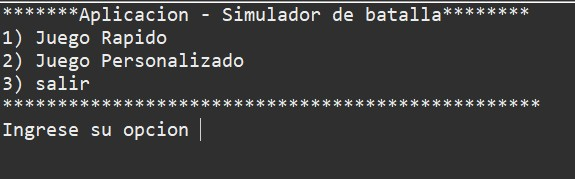
\includegraphics[scale=1]{img/captura 1.jpeg} 
		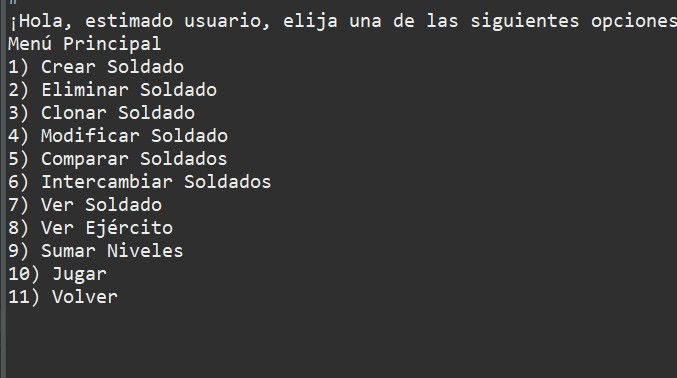
\includegraphics[scale=1]{img/captura 2.jpeg} 
	\end{itemize}

	\subsection{CODIGO FUENTE}
	\begin{itemize}	
		\item Se crea la clase soldado.java
		\item Se crea la clase principal:   VideJuego_v1_lab12.java

			
	\end{itemize}
	
	\begin{lstlisting}[language=bash,caption={Creando la clase soldado y la clase VideoJuego_v1_lab12}][H]
		vim soldado.java
		  vim VideoJuego_v1_lab12.java
	\end{lstlisting}
	
	\begin{lstlisting}[language=bash,caption={Creando la clase Soldado}][H]
			
	package src;
public class Soldado {
		/*
		 Reusando el codiogo de los anterioes labs
		
			 laboratorio Nro 12 ejercicio 1
			 //clase soldado
			 Autor :Mikhail Gabino Velasque Arcos
			colaboro:---
			tiempo:
			 */
		private String nombre;
		private int nivelAtaque;
		private int nivelDefensa;
		private int nivelVida;
		private int vidaActual;
		private int velocidad;
		private int fila;
		private int columna;
		private String actitud;
		private boolean vive;

		public Soldado(String nombre, int fila, int columna){
			this.nombre = nombre;
			this.fila = fila;
			this.columna = columna;
			int vAleat = (int)(Math.random() * 5 + 1);
			vidaActual = vAleat;
			vAleat = (int)(Math.random() * 5 + 1);
			nivelAtaque = vAleat;
			vAleat = (int)(Math.random() * 5 + 1);
			nivelDefensa = vAleat;
			actitud = "defensiva";
			vive = true;
		}
		public Soldado(){
			nombre = "Todos";
			nivelAtaque = 0;
			nivelDefensa = 0;
			nivelVida = 0;
			fila = -1;
			columna = -1;
		}
		public void atacar(){
			actitud = "ofensiva";
			avanzar();
			velocidad++;
		}
		public void defender(){
			actitud = "defensiva";
			velocidad = 0;
		}
		public void avanzar(){
		
		}
		public void retroceder(){
			if(velocidad > 0){
				defender();
			}else{
				velocidad--;
			}
		}
		public void serAtacado(){
			vidaActual--;
			if(vidaActual <= 0){
				morir();
			}
		}
		public void huir(){
			actitud = "fuga";
		}
		public void morir(){
			vive = false;
		}
		public void setVidaActual(int n){
			vidaActual = n;
		}
		public int getVidaActual(){
			return vidaActual;
		}
		public boolean estaVivo(){
			return vive;
		}
		public String getNombre(){
			return nombre;
		}
		public int getFila(){
			return fila;
		}
		public int getColumna(){
			return columna;
		}
		public void setFila(int f){
			fila = f;
		}
		public void setColumna(int c){
			columna = c;
		}

		public Soldado clonarSoldado() {
	    		Soldado nuevoSoldado = new Soldado(nombre, fila, columna);
	    		nuevoSoldado.nivelAtaque = nivelAtaque;
	   		nuevoSoldado.nivelDefensa = nivelDefensa;
	    		nuevoSoldado.nivelVida = nivelVida;
	    		nuevoSoldado.vidaActual = vidaActual;
	    		nuevoSoldado.velocidad = velocidad;
	    		nuevoSoldado.actitud = actitud;
	    		nuevoSoldado.vive = vive;
	    		return nuevoSoldado;
		}

		public String toString() {
			char[] aux = {'A','B','C','D','E','F','G','H','I','J'};
	    	return "Nombre: " + nombre + "\n" +
	          	 	"Nivel de Ataque: " + nivelAtaque + "\n" +
	           		"Nivel de Defensa: " + nivelDefensa + "\n" +
	           		"Vida Actual: " + vidaActual + "\n" +
	           		"Velocidad: " + velocidad + "\n" +
	          		"Fila: " + (fila+1) + "\n" +
	           		"Columna: " + aux[columna] + "\n" +
	           		"Actitud: " + actitud + "\n" +
	           		"Vive: " + vive + "\n";
		}
		public void setNivelAtaque(int n){
			nivelAtaque = n;
		}
		public void setNivelDefensa(int n){
			nivelDefensa = n;
		}
		public int getNivelAtaque(){
			return nivelAtaque;
		}
		public int getNivelDefensa(){
			return nivelDefensa;
		}
		public int getNivelVida(){
			return nivelVida;
		}
		public void comparar(Soldado otroSoldado) {
		    System.out.println("Comparación de atributos con " + otroSoldado.getNombre() + ":");

		    if (!this.nombre.equals(otroSoldado.getNombre())) {
			System.out.println("Nombre: Diferente.");
		    } else {
			System.out.println("Nombre: Igual.");
		    }

		    if (this.nivelAtaque == otroSoldado.getNivelAtaque()) {
			System.out.println("Nivel de Ataque: Igual.");
		    } else {
			System.out.println("Nivel de Ataque: Diferente.");
		    }

		    if (this.nivelDefensa == otroSoldado.getNivelDefensa()) {
			System.out.println("Nivel de Defensa: Igual.");
		    } else {
			System.out.println("Nivel de Defensa: Diferente.");
		    }

		    if (this.vidaActual == otroSoldado.getVidaActual()) {
			System.out.println("Vida Actual: Igual.");
		    } else {
			System.out.println("Vida Actual: Diferente.");
		    }

		    if (this.vive == otroSoldado.estaVivo()) {
			System.out.println("Vive: Igual.");
		    } else {
			System.out.println("Vive: Diferente.");
		    }
		}
		public Soldado sumar(Soldado otroSoldado) {
			this.nivelAtaque += otroSoldado.nivelAtaque;
			this.nivelDefensa += otroSoldado.nivelDefensa;
			this.vidaActual += otroSoldado.vidaActual;
			this.velocidad += otroSoldado.velocidad;
			return this;
	    	}

	}

	
	\end{lstlisting}	
	\begin{lstlisting}[language=bash,caption={Creando la clase principal de VideoJuego_v1_lab12.java}][H]
	
	package src;
import java.util.*;

public class Videojuego_v1_lab12 {
	/*	
		 laboratorio Nro 12 ejercicio 1
		 //clase principal
		 Autor :Mikhail Gabino Velasque Arcos
		colaboro:---
		tiempo:
		 */

	public static void main(String[] args) {
        Scanner entrada = new Scanner(System.in);
        int opt = -1;
        do {
            System.out.println("*******Aplicacion - Simulador de batalla********");
            System.out.println("1) Juego Rapido");
            System.out.println("2) Juego Personalizado");
            System.out.println("3) salir");
            System.out.println("*************************************************");
            System.out.print("Ingrese su opcion ");
            opt = entrada.nextInt();
            
            if (opt == 1) {
                boolean ans = false;
                do {
                    boolean[][] posOcupadas = new boolean[10][10];
                    ArrayList<Soldado> ejercito1 = genEjercito(1, posOcupadas);
                    ArrayList<Soldado> ejercito2 = genEjercito(2, posOcupadas);
                    char[][] tablero = new char[10][10];
                    inicializar(tablero);
                    genTablero(tablero, ejercito1, ejercito2);

                    ans = juegoRapido(tablero, ejercito1, ejercito2);
                } while (ans);
            } else if (opt == 2) {
                boolean[][] posOcupadas = new boolean[10][10];
                ArrayList<Soldado> ejercito1 = genEjercito(1, posOcupadas);
                ArrayList<Soldado> ejercito2 = genEjercito(2, posOcupadas);
                char[][] tablero = new char[10][10];
                inicializar(tablero);
                genTablero(tablero, ejercito1, ejercito2);
                int bomb = -1;
                do {
                    System.out.println("Ingrese el signo del ejercito a personalizar");
                    char c = entrada.next().charAt(0);
                    if (c == '#') {
                        bomb = personalizacion(ejercito1, ejercito2);
                    } else {
                        bomb = personalizacion(ejercito2, ejercito1);
                    }
                } while (bomb == 0);
                if (bomb == 1) {
                    boolean ans = false;
                    do {
                        ans = juegoRapido(tablero, ejercito1, ejercito2);
                    } while (ans);
                } else {
                    // no hace nada
                }
            } else if (opt == 3) {
                System.out.println("Saliendo de la aplicacion");
            } else {
                System.out.println("Opcion no valida");
            }
        } while (opt != 3);
    }

	public static boolean juegoRapido(char[][] tablero, ArrayList<Soldado> ejercito1, ArrayList<Soldado> ejercito2) {
	    Scanner entrada = new Scanner(System.in);
	    System.out.println("******************************************************************");
	    int aux = 0; // nos sirve para determinar que turno actual
	    imprimirTablero(tablero);
	    while (true) {
	        if (aux % 2 == 0) {
	            System.out.println("TURNO DEL EJERCITO #");
	            if (realizarTurno(ejercito1, ejercito2, tablero)) {
	                return true;
	            }
	        } else {
	            System.out.println("TURNO DEL EJERCITO $");
	            if (realizarTurno(ejercito2, ejercito1, tablero)) {
	                return true;
	            }
	        }
	        if (winner(tablero, ejercito1, ejercito2)) {
	            return true;
	        }
	        aux++;
	    }
	}

	public static boolean realizarTurno(ArrayList<Soldado> ejercitoAtacante, ArrayList<Soldado> ejercitoDefensor, char[][] tablero) {
	    ArrayList<Integer> opt = recibirDatos(ejercitoAtacante, ejercitoDefensor);
	    if (opt.size() == 1) {
	        return opt.get(0) == 1;
	    }

	    int axisX = opt.get(0);
	    int axisY = opt.get(1);
	    int toaxisX = opt.get(2);
	    int toaxisY = opt.get(3);

	    System.out.println("El soldado a mover es:");
	    Soldado soldadoSelec = findSoldado(axisX, axisY, ejercitoAtacante);
	    System.out.println(soldadoSelec);
	    
	    moverSoldado(ejercitoAtacante, ejercitoDefensor, soldadoSelec, toaxisX, toaxisY);
	    inicializar(tablero);
	    genTablero(tablero, ejercitoAtacante, ejercitoDefensor);
	    imprimirTablero(tablero);

	    return false;
	}
		public static int menu2(){
			System.out.println("Que accion desea realizar?");
			System.out.println("1) Empezar un juego totalmente nuevo");
			System.out.println("2) Salir al menu");
			Scanner entrada = new Scanner(System.in);
			int opcion = entrada.nextInt();
			return opcion;
		}
		public static ArrayList<Soldado> genEjercito(int w, boolean[][] posOcupadas){
			int num = (int)(Math.random()*10 + 1);
			ArrayList<Soldado> e = new ArrayList<Soldado>();
			for(int i = 0; i < num; i++){
				String nombre = "Soldado"+i+"X"+w;
				int fila = 0;
				int columna = 0;
				do{
					fila = (int)(Math.random()*10);
					columna = (int)(Math.random()*10);
				}while(posOcupadas[fila][columna]);

				posOcupadas[fila][columna] = true;
				Soldado s = new Soldado(nombre, fila, columna);
				e.add(s);
			}	
			return e;
		}
		
		public static void genTablero(char[][] tablero, ArrayList<Soldado> e1, ArrayList<Soldado> e2){
			for(Soldado s: e1){
				int fila = s.getFila();
				int columna = s.getColumna();
				if(s.estaVivo()){
					tablero[fila][columna] = '#';
				}
			}
			for(Soldado s: e2){
				int fila = s.getFila();
				int columna = s.getColumna();
				if(s.estaVivo()){
					tablero[fila][columna] = '$';
				}
			}
		}
		public static void imprimirTablero(char[][] tablero){
			char[] aux = {'A','B','C','D','E','F','G','H','I','J'};
			for(char c: aux){
				System.out.print("\t"+c);
			}
			System.out.println();
			for(int i = 0; i < 10; i++){
				System.out.print(i+1 + "\t");
				for(int j = 0; j < 10; j++){
					System.out.print(tablero[i][j]+"\t");
				}
				System.out.println();
			}
		}
		public static boolean winner(char[][] tablero, ArrayList<Soldado> e1, ArrayList<Soldado> e2){
	    	boolean vivosE1 = false;
	    	boolean vivosE2 = false;

	    	for (Soldado s : e1) {
	        	if (s.estaVivo()) {
	            	vivosE1 = true;
	            	break; 
	        	}
	    	}

	    	for (Soldado s : e2) {
	        	if (s.estaVivo()) {
	            	vivosE2 = true;
	            	break; 
	        	}
	    	}

	    	if (vivosE1 && !vivosE2) {
	        	System.out.println("El ejército # gana la batalla");
	    	} else if (!vivosE1 && vivosE2) {
	        	System.out.println("El ejército $ gana la batalla");
	    	}
	    	return !vivosE1 || !vivosE2;
		}


	    public static void mostrar(ArrayList<Soldado> e) {
	        for (int i = 0; i < e.size(); i++) {
	            System.out.println(e.get(i));
	        }
	    }

	    public static Soldado findSoldado(int axisX, int axisY, ArrayList<Soldado> e){
			for(Soldado s: e){
				if(s.getFila() == axisX && s.getColumna() == axisY && s.estaVivo()){
					return s;
				}
			}

			return null;
	    }
	    public static void inicializar(char [][] tablero){
			for(int i = 0; i < 10; i++){
				for(int j = 0; j < 10; j++){
					tablero[i][j] = '.';
				}
			}
	    }
	    public static void moverSoldado(ArrayList<Soldado> aliado, ArrayList<Soldado> enemigo, Soldado m, int toX, int toY){
	    	//Este metodo mueve el soldado m ()
			//Ahora los datos esta correctamente validados.
			Soldado enem = findSoldado(toX, toY, enemigo);
			if(enem == null){
				//no hay enemigos, realizando movimiento
				m.setFila(toX);
				m.setColumna(toY);
			}else{
				System.out.println("Batalla! -> " + m.getNombre() + ": "+m.getVidaActual() +" vs " + enem.getNombre()+": "+enem.getVidaActual());
				batalla(m, enem, toX, toY);
			}
		
	    }

		public static void batalla(Soldado amigo, Soldado enemigo, int x, int y) {
	    	int vidaTotal = amigo.getVidaActual() + enemigo.getVidaActual();
	    
	   		// Calcula las probabilidades de victoria basadas en la vida actual de los soldados
	    	double probAmigo = (double)amigo.getVidaActual() / vidaTotal * 100.0;
	    	double probEnemigo = (double)enemigo.getVidaActual() / vidaTotal * 100.0;

	    	System.out.println("Probabilidades de victoria:");
	    	System.out.println(amigo.getNombre() + ": " + probAmigo + "%");
	    	System.out.println(enemigo.getNombre() + ": " + probEnemigo + "%");
		
	    	// Realiza la batalla y actualiza las vidas
	    	if (Math.random() * 100 < probAmigo) {
	        	System.out.println("Gana el soldado " + amigo.getNombre());
	        	amigo.setVidaActual(amigo.getVidaActual() + 1);
	        	enemigo.morir();
	        	amigo.setFila(x);
	        	amigo.setColumna(y);
	    	} else {
	        	System.out.println("Gana el soldado " + enemigo.getNombre());
	        	enemigo.setVidaActual(enemigo.getVidaActual() + 1);
	        	amigo.morir();
	    	}
		
	    }
		public static boolean validarOpcion(int x, int y, ArrayList<Soldado> amigos, ArrayList<Soldado> enemigos){
			if(0 <= x && x <= 9 && 0 <= y && y <= 9){
				if(findSoldado(x, y, amigos) != null){
					System.out.println("El soldado escogido es correcto");
					return true;
				}else if(findSoldado(x,y, enemigos) != null){
					System.out.println("El soldado pertenece al ejercito enemigo!. Ingrese de nuevo");
					return false;
				}else{
					System.out.println("No existe!!!");
					return false;
				}
			}else{
				System.out.println("Limites excedidos, ingrese valores adecuados!");
				return false;
			}
		}

		public static boolean validarDestino(int x, int y, ArrayList<Soldado> amigos, ArrayList<Soldado> enemigos){
			if((0 <= x && x <= 9) && (0 <= y && y <= 9)){
				if(findSoldado(x, y, amigos) != null){
					System.out.println("Hay un aliado en el destino, ingrese de nuevo.");
					return false;
				}else if(findSoldado(x,y, enemigos) != null){
					System.out.println("Soldado enemigo encontrado, iniciando batalla!!!");
					return true;
				}else{
					System.out.println("Moviendose a la ubicacion");
					return true;
				}
			}else{
				System.out.println("Limites excedidos, ingrese valores adecuados!");
				return false;
			}
		}
		public static boolean validarEleccion(int x, int y, ArrayList<Soldado> amigos, ArrayList<Soldado> enemigos){
			//retorna true si no hay soldados
			if(0 <= x && x <= 9 && 0 <= y && y <= 9){
				if(findSoldado(x, y, amigos) == null){
					System.out.println("Posicion vacia");
					return true;
				}else if(findSoldado(x,y, enemigos) == null){
					System.out.println("Posicion vacial");
					return true;
				}else{
					System.out.println("Ocupado");
					return false;
				}
			}else{
				System.out.println("Limites excedidos, ingrese valores adecuados!");
				return false;
			}
			
		}
		public static ArrayList<Integer> recibirDatos(ArrayList<Soldado> amigo, ArrayList<Soldado> enemigo){
			ArrayList<Integer> datos = new ArrayList<Integer>();
			Scanner entrada = new Scanner(System.in);
			int axisX = 0;
			int axisY = 0;
			int toaxisX = 0;
			int toaxisY = 0;
			boolean s = false;
			do{	
				System.out.print("Ingrese las coordenadas del soldado que desea mover. Si desea cancelar el juego, escriba salir: ");
				String g = entrada.nextLine();
				if(g.equals("salir")){
					s = true;
					break;
				}else{
					axisX = Integer.parseInt(g.substring(0, g.indexOf(" ")));
					axisY = Integer.parseInt(g.substring(g.indexOf(" ")+1));
					axisX--;
					axisY--;
				}
			}while(!validarOpcion(axisX, axisY, amigo, enemigo));
				if(s){
					int op = menu2();
					datos.clear();
					datos.add(op);
					return datos; 
				}
			datos.add(axisX);
			datos.add(axisY);
			s = false;
			do{
				System.out.print("Ingrese las coordenadas del destino. Si desea cancelar el juego, escriba salir: ");
				String g = entrada.nextLine();
				if(g.equals("salir")){
					s = true;
					break;
				}else{
					toaxisX = Integer.parseInt(g.substring(0, g.indexOf(" ")));
					toaxisY = Integer.parseInt(g.substring(g.indexOf(" ")+1));
					toaxisX--;
					toaxisY--;
				}
			}while(!validarDestino(toaxisX, toaxisY, amigo, enemigo));
				if(s){
					int op = menu2();
					datos.clear();
					datos.add(op);
					return datos; 
				}
			datos.add(toaxisX);
			datos.add(toaxisY);
			return datos;
		
		}
		public static int personalizacion(ArrayList<Soldado> e, ArrayList<Soldado> o){
			Scanner entrada = new Scanner(System.in);
			System.out.println("¡Hola, estimado usuario, elija una de las siguientes opciones");
	        System.out.println("Menú Principal");
	        System.out.println("1) Crear Soldado");
	        System.out.println("2) Eliminar Soldado");
	        System.out.println("3) Clonar Soldado");
	        System.out.println("4) Modificar Soldado");
	        System.out.println("5) Comparar Soldados");
	        System.out.println("6) Intercambiar Soldados");
	        System.out.println("7) Ver Soldado");
	        System.out.println("8) Ver Ejército");
	        System.out.println("9) Sumar Niveles");
	        System.out.println("10) Jugar");
	        System.out.println("11) Volver");
			int v = entrada.nextInt();
			while(true){
				if(v == 1){
					if(e.size() < 10){
						System.out.println("Ingrese el nombre: ");
						String n = entrada.next();
						int arr[] = recibirPos2(e, o);
						int x = arr[0];
						int y = arr[1];

						Soldado s = new Soldado(n, x, y);
						e.add(s);
					}else{
						System.out.println("El ejercito esta lleno!!!");
					}
					break;
				}else if(v == 2){
					if(e.size() > 1){
						int arr[] = recibirPos1(e, o);
						int x = arr[0];
						int y = arr[1];
						e.remove(findSoldado(x,y, e));
					}else{
						System.out.println("El ejercito no puede estar vacio!!!");
					}
					break;

				}else if(v == 3){
					if(e.size() < 10){
						int arr[] = recibirPos1(e, o);
						int x = arr[0];
						int y = arr[1];
						Soldado s = findSoldado(x,y,e).clonarSoldado();

						System.out.println("Ingrese la nueva posicion");
						int arr2[] = recibirPos2(e, o);
						x = arr2[0];
						y = arr2[1];
						s.setFila(x);
						s.setColumna(y);
						e.add(s);
					}else{
						System.out.println("El ejercito esta lleno!!!");
					}
					break;

				}else if(v == 4){
					System.out.println("Ingrese las coordenadas del soldado a verificar!");
					int arr[] = recibirPos1(e, o);
					int x = arr[0];
					int y = arr[1];
					Soldado s = findSoldado(x,y,e);
					menu3(s);
					break;
				}else if(v == 5){
					
					System.out.println("Ingrese las coordenadas del primer soldado");
					int arr1[] = recibirPos1(e, o);
					int x = arr1[0];
					int y = arr1[1];
					Soldado s1 = findSoldado(x, y, e);

					System.out.println("Ingrese las coordenadas del segundo soldado");
					int arr2[] = recibirPos1(e, o);
					x = arr2[0];
					y = arr2[1];
					Soldado s2 = findSoldado(x, y, e);

					s1.comparar(s2);
					break;

				}else if(v == 6){
					System.out.println("Ingrese las coordenadas del primer soldado");
					int arr1[] = recibirPos1(e, o);
					int x = arr1[0];
					int y = arr1[1];
					Soldado s1 = findSoldado(x, y, e);

					System.out.println("Ingrese las coordenadas del segundo soldado");
					int arr2[] = recibirPos1(e, o);
					x = arr2[0];
					y = arr2[1];
					Soldado s2 = findSoldado(x, y, e);

					int index1 = -1;
					int index2 = -1;
					for(int i = 0; i < e.size(); i++){
						if(e.get(i) == s1){
							index1 = i;
						}
						if(e.get(i) == s2){
							index2 = i;
						}
					}

					Soldado temp = s1.clonarSoldado();
					e.remove(index2);
					e.add(index1, s2);

					e.remove(index1);
					e.add(index2, temp);
					break;

				}else if(v == 7){
					System.out.println("Ingrese el nombre del soldado a buscar: ");	
					String n = entrada.next();
					int index = -1;
					for(int i = 0; i < e.size(); i++){
						if(e.get(i).getNombre().equals(n)){
							index = i;
						}
					}	
					if(index != -1){
						System.out.println("Se encontro ese soldado.");
						System.out.println(e.get(index));
					}
					break;
				}else if(v == 8){
					System.out.println("Mostrando ejercito ");		
					mostrar(e);
					break;
				}else if(v == 9){
					Soldado soldTemp = new Soldado();
					for(Soldado s: e){
						soldTemp = soldTemp.sumar(s);
					}
					System.out.println("Suma de niveles:");
	        		System.out.println("Nivel de Ataque: " + soldTemp.getNivelAtaque());
	        		System.out.println("Nivel de Defensa: " + soldTemp.getNivelDefensa());
	        		System.out.println("Nivel de Vida: " + soldTemp.getNivelVida());
					break;
				}else if(v == 10){
					return 1;
				}else if(v == 11){
					return 2;
				}
				System.out.println("Algo salio mal, intente de nuevo!");

			}
			return 0;
		}
		//lee datos de un soldado en el ejercito
		public static int[] recibirPos1(ArrayList<Soldado> e, ArrayList<Soldado> o){
			Scanner sc = new Scanner(System.in);
			int arr[] = new int[2];
			do{
				System.out.print("Ingrese la fila del soldado: ");
				arr[0] = sc.nextInt();
				System.out.print("Ingrese la columna del soldado: ");
				arr[1] = sc.nextInt();
				arr[0]--;
				arr[1]--;
			}while(!validarOpcion(arr[0],arr[1],e,o));
			return arr;
		}
		//recibe datos de un espacio vacio
		public static int[] recibirPos2(ArrayList<Soldado> e, ArrayList<Soldado> o){
			Scanner sc = new Scanner(System.in);
			int arr[] = new int[2];
			do{
				System.out.print("Ingrese la fila del soldado: ");
				arr[0] = sc.nextInt();
				System.out.print("Ingrese la columna del soldado: ");
				arr[1] = sc.nextInt();
				arr[0]--;
				arr[1]--;	
			}while(!validarEleccion(arr[0],arr[1],e,o));
			return arr;
		}

		public static void menu3(Soldado s){
			System.out.println("¿Que desea modificar?");
			System.out.println("1) Nivel de Ataque");
			System.out.println("2) Nivel de Defensa");
			System.out.println("3) Nivel de Vida");
			Scanner sc = new Scanner(System.in);
			int o = sc.nextInt();
			if(o == 1){
				System.out.print("Ingrese el nuevo valor del ataque: ");
				int n = sc.nextInt();
				s.setNivelAtaque(n);
				
			}else if(o == 2){
				System.out.print("Ingrese el nuevo valor de la defensa: ");
				int n = sc.nextInt();
				s.setNivelDefensa(n);
			}else if(o == 3){
			
				System.out.print("Ingrese el nuevo valor de la vida: ");
				int n = sc.nextInt();
				s.setVidaActual(n);
			}
		}
	} 



				\end{lstlisting}
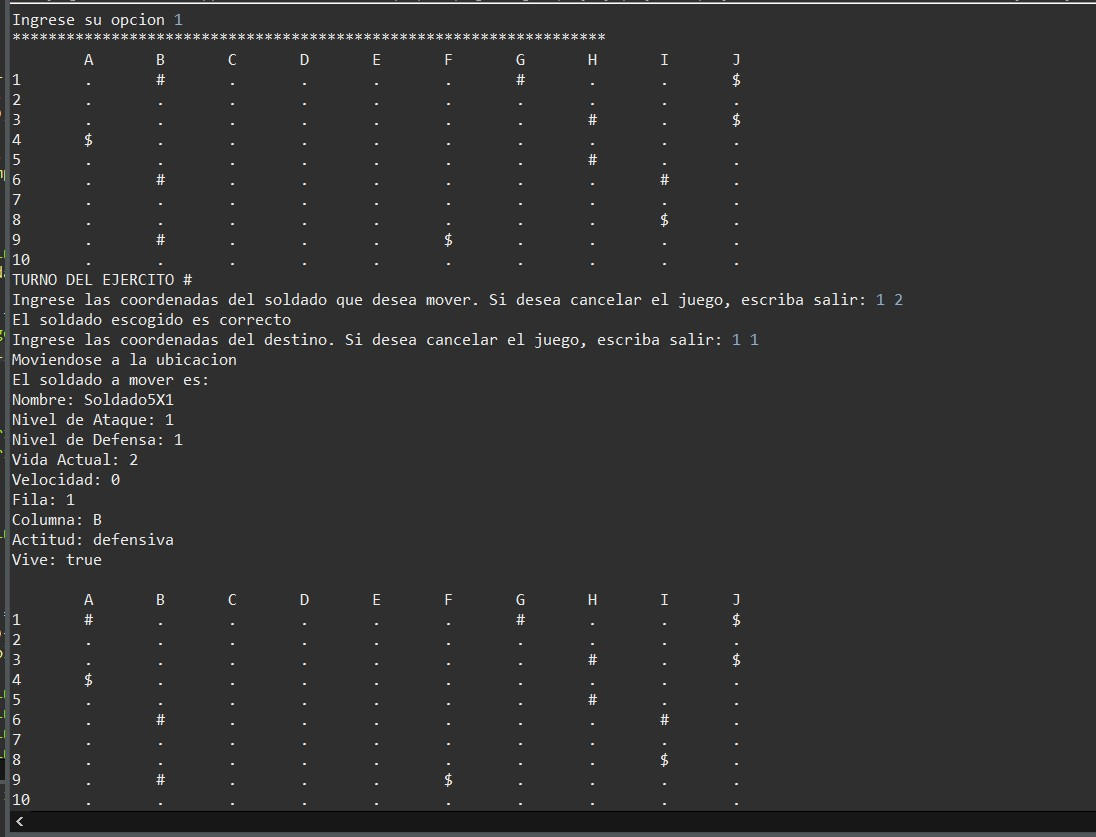
\includegraphics[scale=0.50]{img/captura 3.jpeg} 
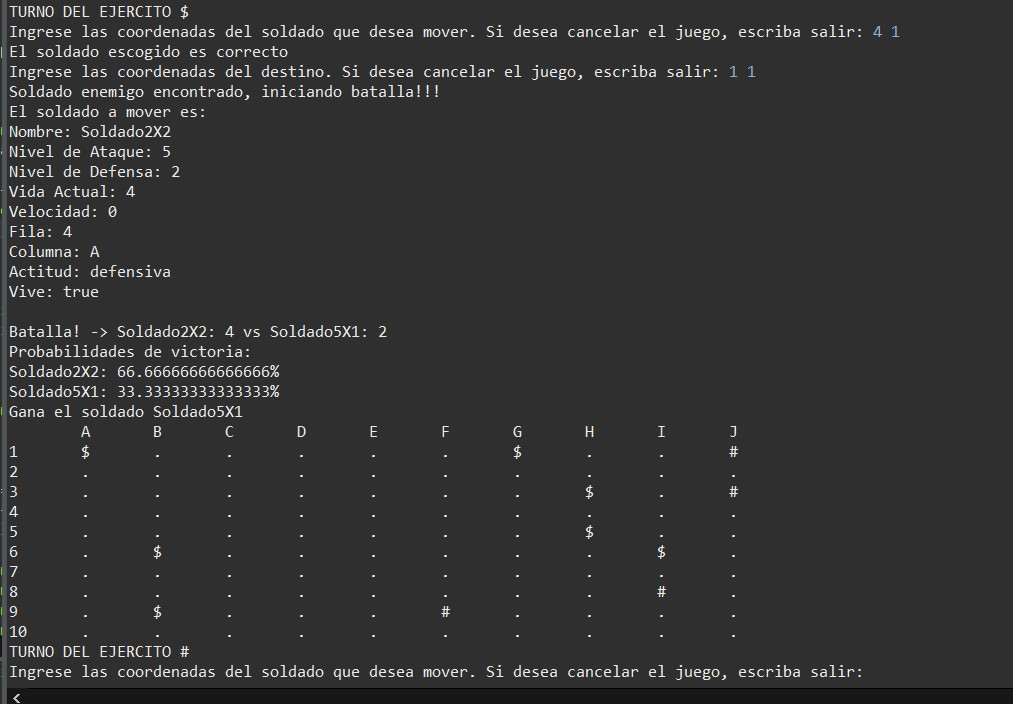
\includegraphics[scale=0.50]{img/captura 4.jpeg} 
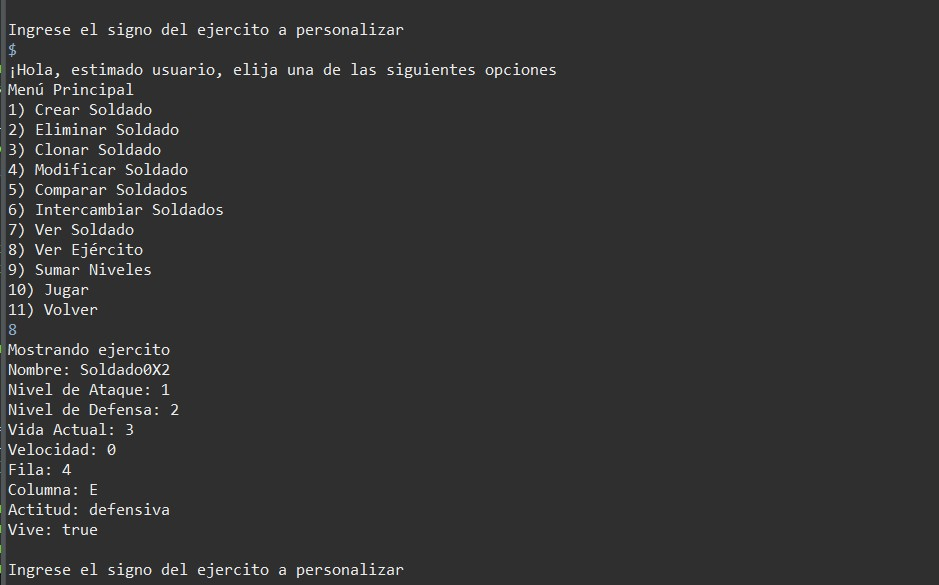
\includegraphics[scale=0.50]{img/captura 5.jpeg} 
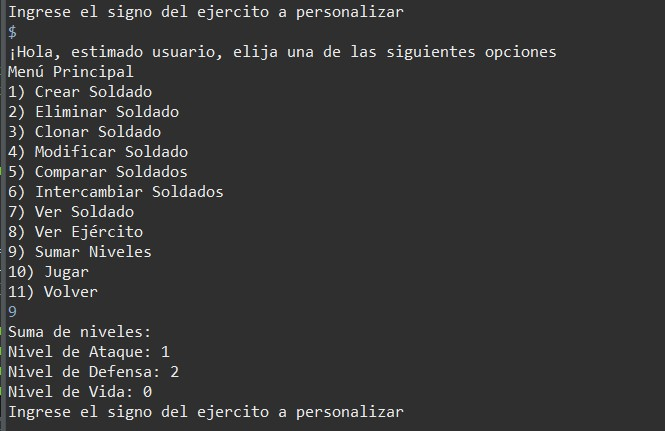
\includegraphics[scale=0.50]{img/captura 6.jpeg} 

\includegraphics[scale=1]{img/logo_abet.png} 

\end{document}